\documentclass[11pt]{article}
\usepackage[utf8]{inputenc}
\usepackage{settings}


\title{Heat Lens Results}
\date{}

\begin{document}

\maketitle

\tableofcontents

\pagebreak
\section{Numerical Results}
\subsection{Single Flux}
\begin{figure}[!h]
    \centering
    \begin{tabular}{|c|c||c|c|}\hline
    $\alpha$ & $1$ & $V_{\theta_1}$ & unbound \\\hline
    $\beta$ & $0.1$ & $ds$ & $0.1$ \\\hline
    \end{tabular}
    \caption{Single Flux}
\end{figure}
\begin{figure}[!h]
    \begin{tabular}{cc}
         \frame{
\includegraphics[scale=.5,clip,trim={10 10 10 10}]{img/singleFlux/dirichlet_conditions.pdf}}&
         \frame{
\includegraphics[scale=.5,clip,trim={10 10 10 10}]{img/singleFlux/neumann_conditions.pdf}}
         \\
         Conducting Window & Boundary Flux \\
          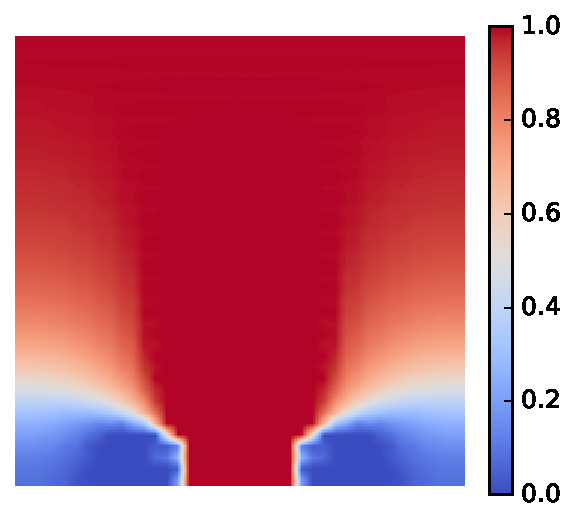
\includegraphics[scale=.5]{img/singleFlux/theta.pdf}&
         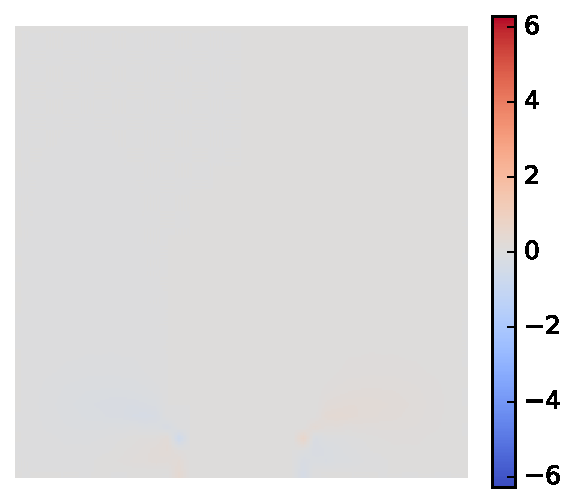
\includegraphics[scale=.5]{img/singleFlux/phi.pdf}
         \\
         $\theta $ & $\phi$ 
    \end{tabular}
\end{figure}
\pagebreak
\begin{figure}[!h]
    \begin{tabular}{cc}
         \frame{
\includegraphics[scale=.5,clip,trim={10 10 10 10}]{img/singleFlux/A_nabla_u.pdf}}&
         \frame{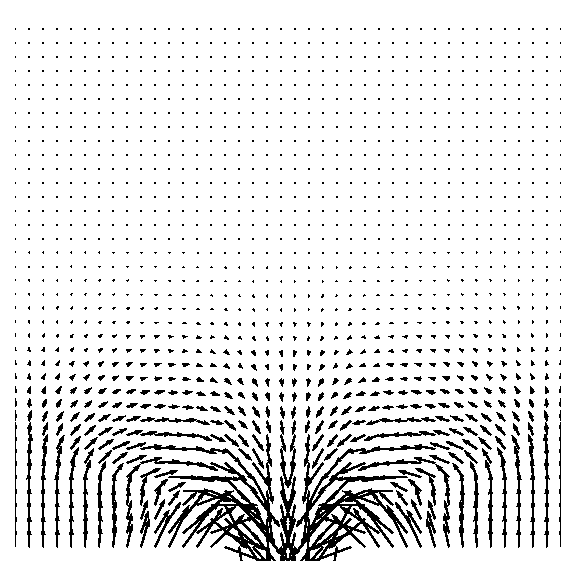
\includegraphics[scale=.5,clip,trim={10 10 10 10}]{img/singleFlux/A_nabla_p.pdf}}
         \\
         $A\nabla u$ & $A \nabla p$ \\
      \frame{
\includegraphics[scale=.5,clip,trim={10 10 10 10}]{img/singleFlux/nabla_u.pdf}}&
         \frame{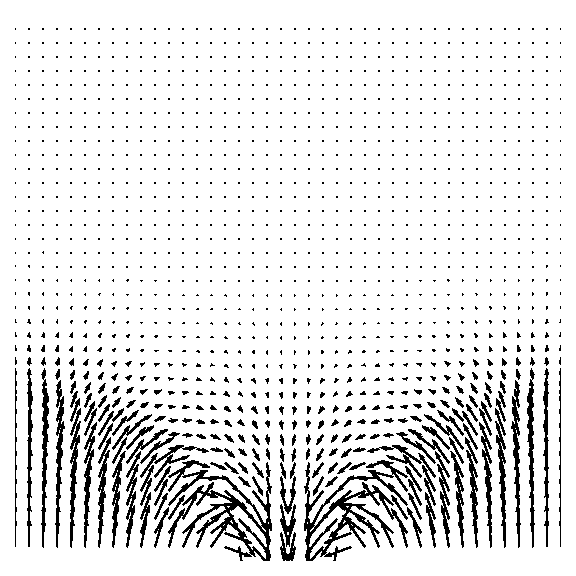
\includegraphics[scale=.5,clip,trim={10 10 10 10}]{img/singleFlux/nabla_p.pdf}}
         \\
         $\nabla u$ & $\nabla p$
    \end{tabular}
\end{figure}
\pagebreak
\begin{figure}[!h]
    \begin{tabular}{cc}
         \frame{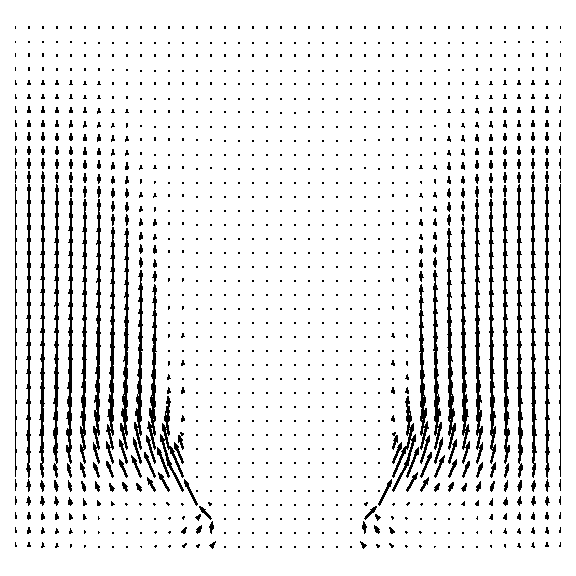
\includegraphics[scale=.5,clip,trim={10 10 10 10}]{img/singleFlux/eig.pdf}}&
         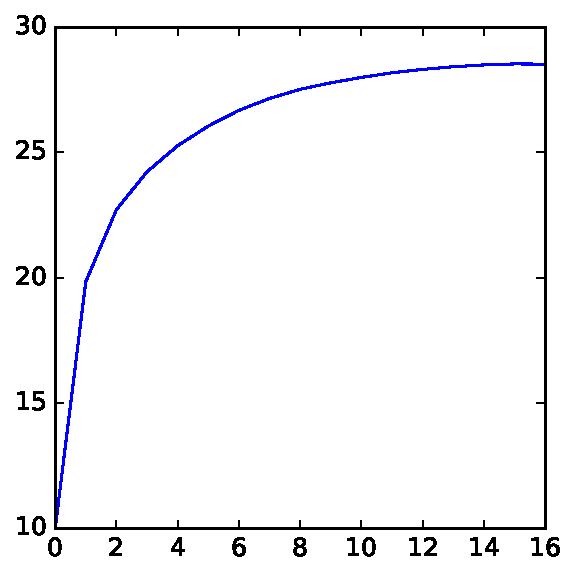
\includegraphics[scale=.5]{img/singleFlux/energy.pdf}
         \\
         $(\lambda_{\max}-\lambda_{\min})v_{\max}$ & $J(A_i,T_i)$ 
    \end{tabular}
\end{figure}

\pagebreak
\subsection{Split Flux}
\begin{figure}[!h]
    \centering
    \begin{tabular}{|c|c||c|c|}\hline
    $\alpha$ & $1$ & $V_{\theta_1}$ & unbound \\\hline
    $\beta$ & $0.1$ & $ds$ & $0.1$ \\\hline
    \end{tabular}
    \caption{Split Flux}
\end{figure}
\begin{figure}[!h]
    \begin{tabular}{cc}
         \frame{
\includegraphics[scale=.5,clip,trim={10 10 10 10}]{img/splitFlux/dirichlet_conditions.pdf}}&
         \frame{
\includegraphics[scale=.5,clip,trim={10 10 10 10}]{img/splitFlux/neumann_conditions.pdf}}
         \\
         Conducting Window & Boundary Flux \\
          \includegraphics[scale=.5]{img/splitFlux/theta.pdf}&
         
\includegraphics[scale=.5]{img/splitFlux/phi.pdf}
         \\
         $\theta $ & $\phi$ 
    \end{tabular}
\end{figure}
\pagebreak
\begin{figure}[!h]
    \begin{tabular}{cc}
         \frame{
\includegraphics[scale=.5,clip,trim={10 10 10 10}]{img/splitFlux/A_nabla_u.pdf}}&
         \frame{\includegraphics[scale=.5,clip,trim={10 10 10 10}]{img/splitFlux/A_nabla_p.pdf}}
         \\
         $A\nabla u$ & $A \nabla p$ \\
      \frame{
\includegraphics[scale=.5,clip,trim={10 10 10 10}]{img/splitFlux/nabla_u.pdf}}&
         \frame{\includegraphics[scale=.5,clip,trim={10 10 10 10}]{img/splitFlux/nabla_p.pdf}}
         \\
         $\nabla u$ & $\nabla p$
    \end{tabular}
\end{figure}
\pagebreak
\begin{figure}[!h]
    \begin{tabular}{cc}
         \frame{\includegraphics[scale=.5,clip,trim={10 10 10 10}]{img/splitFlux/eig.pdf}}&
         \includegraphics[scale=.5]{img/splitFlux/energy.pdf}
         \\
         $(\lambda_{\max}-\lambda_{\min})v_{\max}$ & $J(A_i,T_i)$ 
    \end{tabular}
\end{figure}

\pagebreak
\subsection{Robust Split Flux}
\begin{figure}[!h]
    \centering
    \begin{tabular}{|c|c||c|c|}\hline
    $\alpha$ & $1$ & $V_{\theta_1}$ & unbound \\\hline
    $\beta$ & $0.1$ & $ds$ & $0.1$ \\\hline
    \end{tabular}
    \caption{Robust Split Flux}
\end{figure}
\begin{figure}[!h]
    \begin{tabular}{cc}
         \frame{
\includegraphics[scale=.5,clip,trim={10 10 10 10}]{img/splitFluxRobust/dirichlet_conditions.pdf}}&
         \frame{
\includegraphics[scale=.5,clip,trim={10 10 10 10}]{img/splitFluxRobust/neumann_conditions.pdf}}
         \\
         Conducting Window & Boundary Flux \\
          \includegraphics[scale=.5]{img/splitFluxRobust/theta.pdf}&
         
\includegraphics[scale=.5]{img/splitFluxRobust/phi.pdf}
         \\
         $\theta $ & $\phi$ 
    \end{tabular}
\end{figure}
\pagebreak
\begin{figure}[!h]
    \begin{tabular}{cc}
         \frame{
\includegraphics[scale=.5,clip,trim={10 10 10 10}]{img/splitFluxRobust/A_nabla_u.pdf}}&
         \frame{\includegraphics[scale=.5,clip,trim={10 10 10 10}]{img/splitFluxRobust/A_nabla_p.pdf}}
         \\
         $A\nabla u$ & $A \nabla p$ \\
      \frame{
\includegraphics[scale=.5,clip,trim={10 10 10 10}]{img/splitFluxRobust/nabla_u.pdf}}&
         \frame{\includegraphics[scale=.5,clip,trim={10 10 10 10}]{img/splitFluxRobust/nabla_p.pdf}}
         \\
         $\nabla u$ & $\nabla p$
    \end{tabular}
\end{figure}
\pagebreak
\begin{figure}[!h]
    \begin{tabular}{cc}
         \frame{\includegraphics[scale=.5,clip,trim={10 10 10 10}]{img/splitFluxRobust/eig.pdf}}&
         \includegraphics[scale=.5]{img/splitFluxRobust/energy.pdf}
         \\
         $(\lambda_{\max}-\lambda_{\min})v_{\max}$ & $J(A_i,T_i)$ 
    \end{tabular}
\end{figure}
%%
\pagebreak
\subsection{Split Flux with Volume Constraint}
\begin{figure}[!h]
    \centering
    \begin{tabular}{|c|c||c|c|}\hline
    $\alpha$ & $1$ & $V_{\theta_1}$ & $0.5$ \\\hline
    $\beta$ & $0.1$ & $ds$ & $0.1$ \\\hline
    \end{tabular}
    \caption{Robust Split Flux}
\end{figure}
\begin{figure}[!h]
    \begin{tabular}{cc}
         \frame{
\includegraphics[scale=.5,clip,trim={10 10 10 10}]{img/splitFluxVol/dirichlet_conditions.pdf}}&
         \frame{
\includegraphics[scale=.5,clip,trim={10 10 10 10}]{img/splitFluxVol/neumann_conditions.pdf}}
         \\
         Conducting Window & Boundary Flux \\
          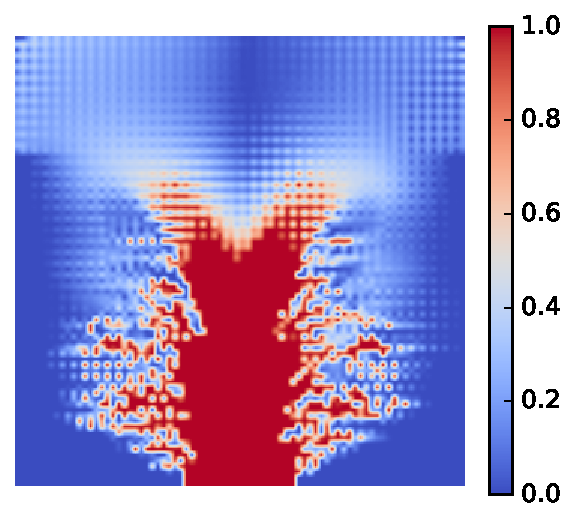
\includegraphics[scale=.5]{img/splitFluxVol/theta.pdf}&
         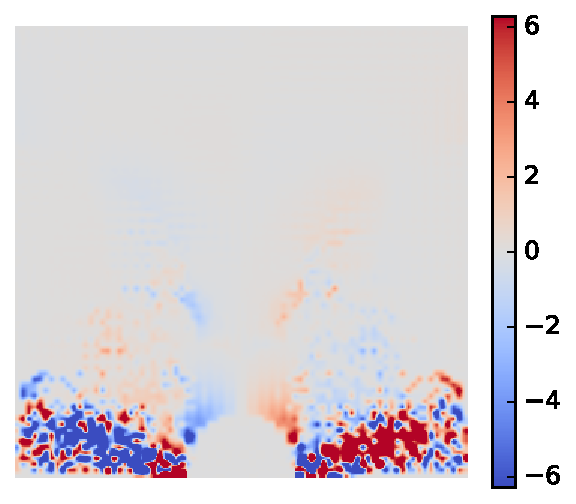
\includegraphics[scale=.5]{img/splitFluxVol/phi.pdf}
         \\
         $\theta $ & $\phi$ 
    \end{tabular}
\end{figure}
\pagebreak
\begin{figure}[!h]
    \begin{tabular}{cc}
         \frame{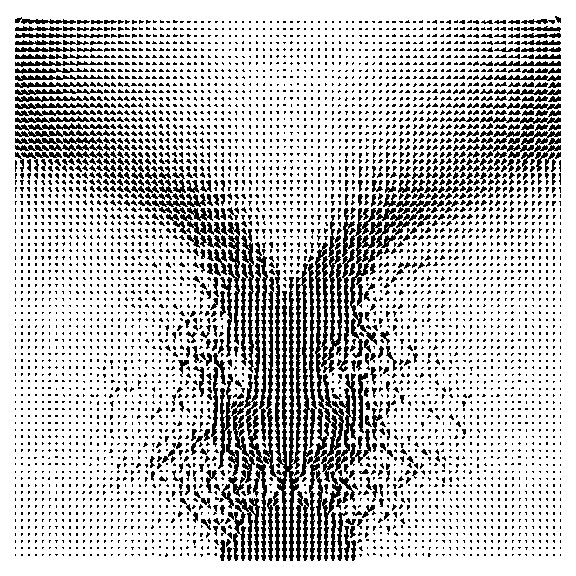
\includegraphics[scale=.5,clip,trim={10 10 10 10}]{img/splitFluxVol/A_nabla_u.pdf}}&
         \frame{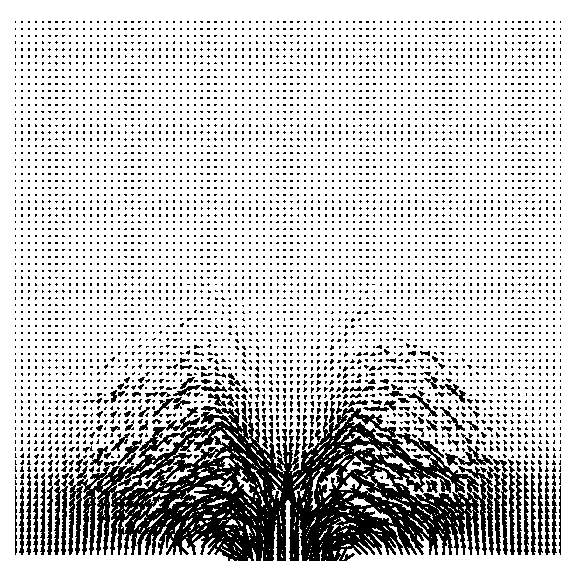
\includegraphics[scale=.5,clip,trim={10 10 10 10}]{img/splitFluxVol/A_nabla_p.pdf}}
         \\
         $A\nabla u$ & $A \nabla p$ \\
      \frame{
\includegraphics[scale=.5,clip,trim={10 10 10 10}]{img/splitFluxVol/nabla_u.pdf}}&
         \frame{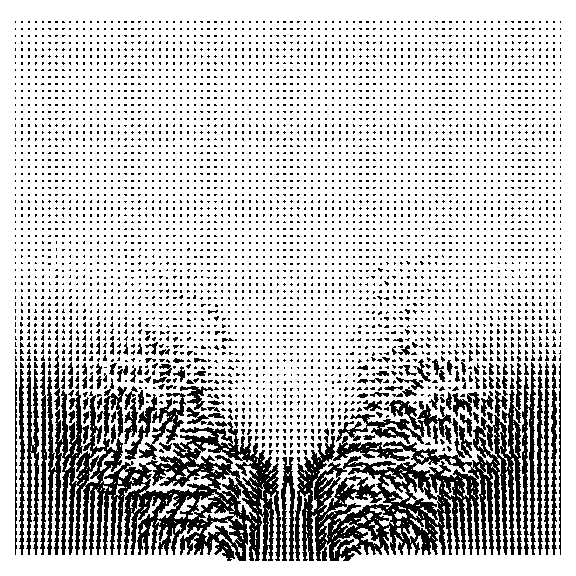
\includegraphics[scale=.5,clip,trim={10 10 10 10}]{img/splitFluxVol/nabla_p.pdf}}
         \\
         $\nabla u$ & $\nabla p$
    \end{tabular}
\end{figure}
\pagebreak
\begin{figure}[!h]
    \begin{tabular}{cc}
         \frame{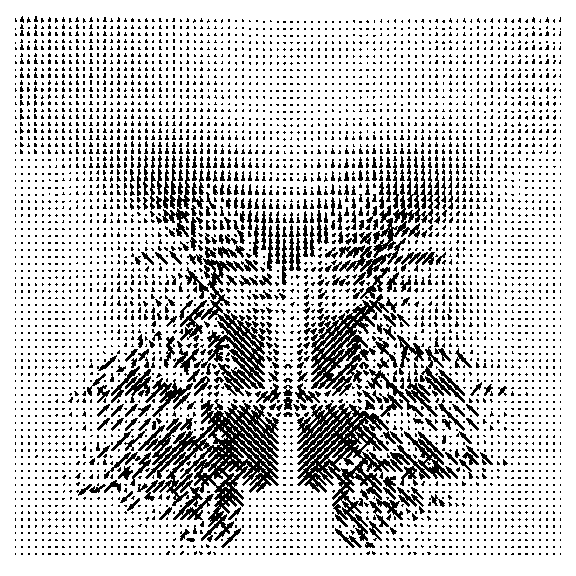
\includegraphics[scale=.5,clip,trim={10 10 10 10}]{img/splitFluxVol/eig.pdf}}&
         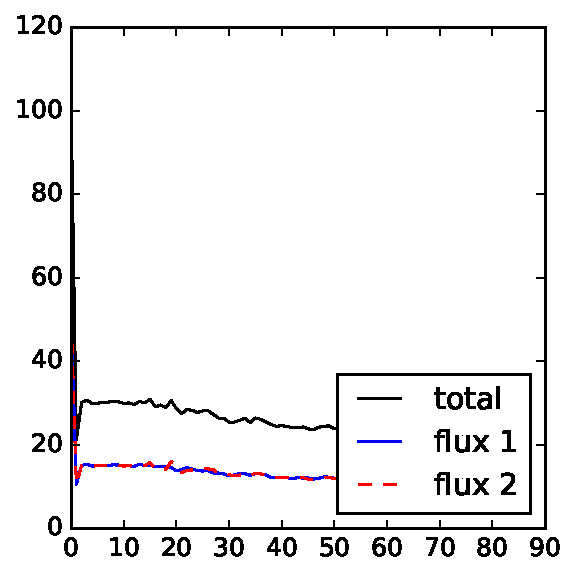
\includegraphics[scale=.5]{img/splitFluxVol/energy.pdf}
         \\
         $(\lambda_{\max}-\lambda_{\min})v_{\max}$ & $J(A_i,T_i)$ 
    \end{tabular}
\end{figure}


\pagebreak
\subsection{Asymmetric Flux}
\begin{figure}[!h]
    \centering
    \begin{tabular}{|c|c||c|c|}\hline
    $\alpha$ & $1$ & $V_{\theta_1}$ & unbound \\\hline
    $\beta$ & $0.5$ & $ds$ & $0.05$ \\\hline
    \end{tabular}
    \caption{Asymmetric Flux}
\end{figure}
\begin{figure}[!h]
    \begin{tabular}{cc}
         \frame{
\includegraphics[scale=.5,clip,trim={10 10 10 10}]{img/asymmetricFlux/dirichlet_conditions.pdf}}&
         \frame{
\includegraphics[scale=.5,clip,trim={10 10 10 10}]{img/asymmetricFlux/neumann_conditions.pdf}}
         \\
         Conducting Window & Boundary Flux \\
          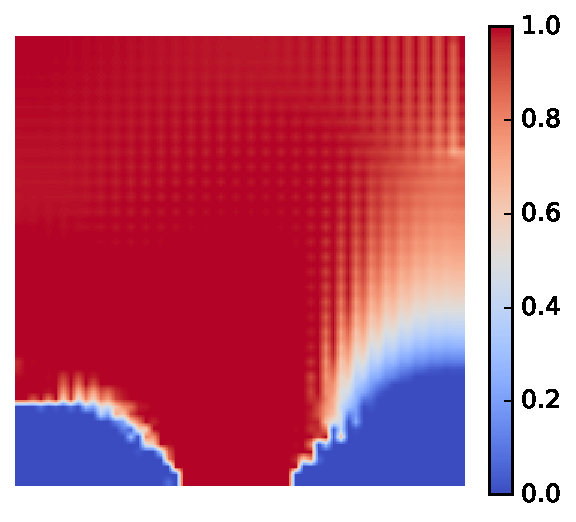
\includegraphics[scale=.5]{img/asymmetricFlux/theta.pdf}&
         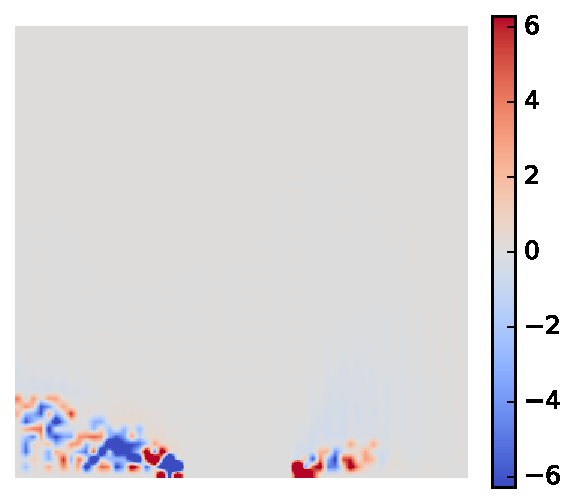
\includegraphics[scale=.5]{img/asymmetricFlux/phi.pdf}
         \\
         $\theta $ & $\phi$ 
    \end{tabular}
\end{figure}
\pagebreak
\begin{figure}[!h]
    \begin{tabular}{cc}
         \frame{
\includegraphics[scale=.5,clip,trim={10 10 10 10}]{img/asymmetricFlux/A_nabla_u.pdf}}&
         \frame{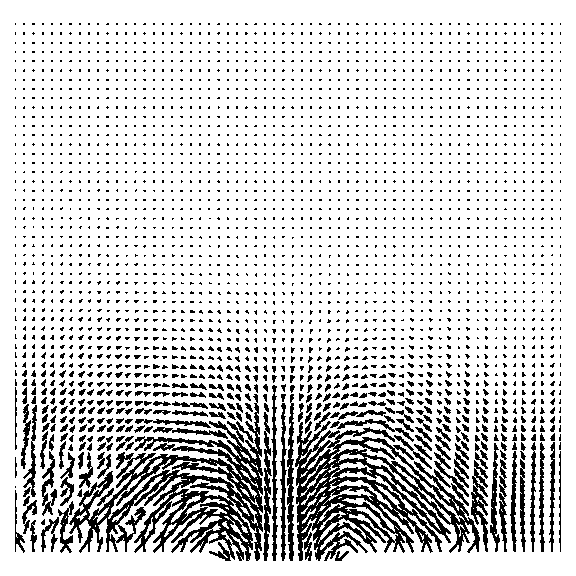
\includegraphics[scale=.5,clip,trim={10 10 10 10}]{img/asymmetricFlux/A_nabla_p.pdf}}
         \\
         $A\nabla u$ & $A \nabla p$ \\
      \frame{
\includegraphics[scale=.5,clip,trim={10 10 10 10}]{img/asymmetricFlux/nabla_u.pdf}}&
         \frame{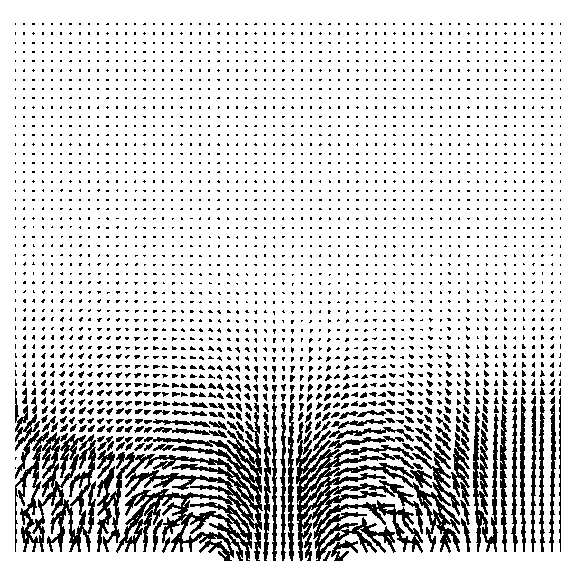
\includegraphics[scale=.5,clip,trim={10 10 10 10}]{img/asymmetricFlux/nabla_p.pdf}}
         \\
         $\nabla u$ & $\nabla p$
    \end{tabular}
\end{figure}
\pagebreak
\begin{figure}[!h]
    \begin{tabular}{cc}
         \frame{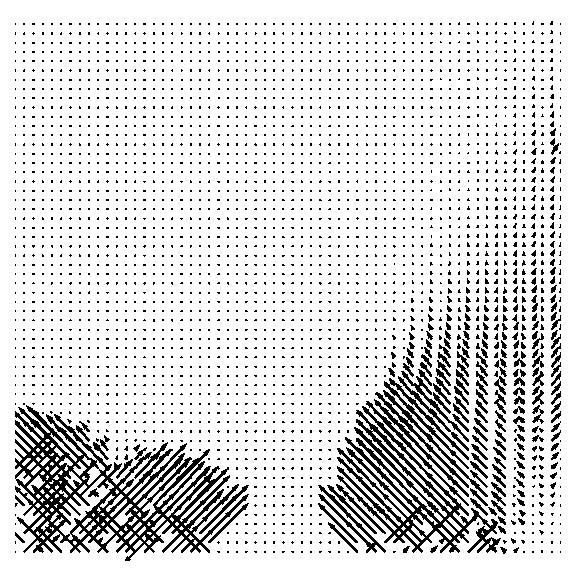
\includegraphics[scale=.5,clip,trim={10 10 10 10}]{img/asymmetricFlux/eig.pdf}}&
         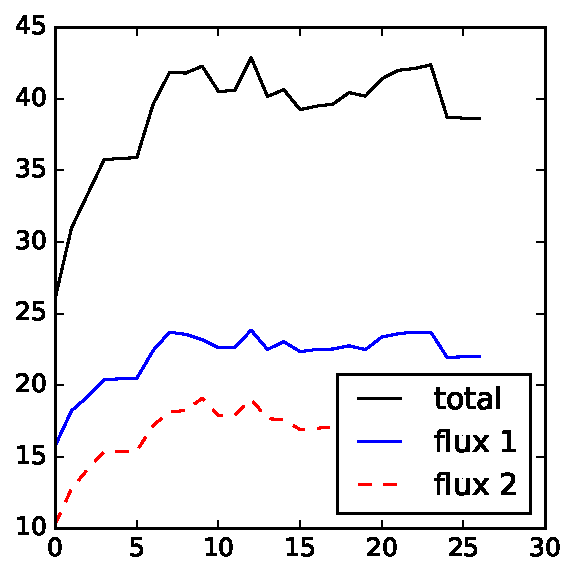
\includegraphics[scale=.5]{img/asymmetricFlux/energy.pdf}
         \\
         $(\lambda_{\max}-\lambda_{\min})v_{\max}$ & $J(A_i,T_i)$ 
    \end{tabular}
\end{figure}

\pagebreak
\subsection{Robust Asymmetric Flux}
\begin{figure}[!h]
    \centering
    \begin{tabular}{|c|c||c|c|}\hline
    $\alpha$ & $1$ & $V_{\theta_1}$ & unbound \\\hline
    $\beta$ & $0.5$ & $ds$ & $0.05$ \\\hline
    \end{tabular}
    \caption{Robust Asymmetric Flux}
\end{figure}
\begin{figure}[!h]
    \begin{tabular}{cc}
         \frame{\includegraphics[scale=.5,clip,trim={10 10 10 10}]{img/asymmetricFluxRobust/dirichlet_conditions.pdf}}&
         \frame{\includegraphics[scale=.5,clip,trim={10 10 10 10}]{img/asymmetricFluxRobust/neumann_conditions.pdf}}
         \\
         Conducting Window & Boundary Flux \\
          \includegraphics[scale=.5]{img/asymmetricFluxRobust/theta.pdf}&
         \includegraphics[scale=.5]{img/asymmetricFluxRobust/phi.pdf}
         \\
         $\theta $ & $\phi$ 
    \end{tabular}
\end{figure}
\pagebreak
\begin{figure}[!h]
    \begin{tabular}{cc}
         \frame{\includegraphics[scale=.5,clip,trim={10 10 10 10}]{img/asymmetricFluxRobust/A_nabla_u.pdf}}&
         \frame{\includegraphics[scale=.5,clip,trim={10 10 10 10}]{img/asymmetricFluxRobust/A_nabla_p.pdf}}
         \\
         $A\nabla u$ & $A \nabla p$ \\
      \frame{\includegraphics[scale=.5,clip,trim={10 10 10 10}]{img/asymmetricFluxRobust/nabla_u.pdf}}&
         \frame{\includegraphics[scale=.5,clip,trim={10 10 10 10}]{img/asymmetricFluxRobust/nabla_p.pdf}}
         \\
         $\nabla u$ & $\nabla p$
    \end{tabular}
\end{figure}
\pagebreak
\begin{figure}[!h]
    \begin{tabular}{cc}
         \frame{\includegraphics[scale=.5,clip,trim={10 10 10 10}]{img/asymmetricFluxRobust/nabla_u1.pdf}}&
         \frame{\includegraphics[scale=.5,clip,trim={10 10 10 10}]{img/asymmetricFluxRobust/nabla_u2.pdf}}
         \\
         $\nabla u_1$ & $\nabla u_2$ \\
      \frame{\includegraphics[scale=.5,clip,trim={10 10 10 10}]{img/asymmetricFluxRobust/A_nabla_u1.pdf}}&
         \frame{\includegraphics[scale=.5,clip,trim={10 10 10 10}]{img/asymmetricFluxRobust/A_nabla_u2.pdf}}
         \\
         $A\nabla u_1$ & $A\nabla u_2$
    \end{tabular}
\end{figure}
\pagebreak
\begin{figure}[!h]
    \begin{tabular}{cc}
         \frame{\includegraphics[scale=.5,clip,trim={10 10 10 10}]{img/asymmetricFluxRobust/eig.pdf}}&
         \includegraphics[scale=.5]{img/asymmetricFluxRobust/energy.pdf}
         \\
         $(\lambda_{\max}-\lambda_{\min})v_{\max}$ & $J(A_i,T_i)$ 
    \end{tabular}
\end{figure}


%%
\pagebreak
\subsection{Robust Asymmetric Flux with Volume Constraint}
\begin{figure}[!h]
    \centering
    \begin{tabular}{|c|c||c|c|}\hline
    $\alpha$ & $1$ & $V_{\theta_1}$ & .5 \\\hline
    $\beta$ & $0.1$ & $ds$ & $0.1$ \\\hline
    \end{tabular}
    \caption{Robust Split Flux}
\end{figure}
\begin{figure}[!h]
    \begin{tabular}{cc}
         \frame{\includegraphics[scale=.5,clip,trim={10 10 10 10}]{img/asymmetricFluxVol/dirichlet_conditions.pdf}}&
         \frame{\includegraphics[scale=.5,clip,trim={10 10 10 10}]{img/asymmetricFluxVol/neumann_conditions.pdf}}
         \\
         Conducting Window & Boundary Flux \\
          \includegraphics[scale=.5]{img/asymmetricFluxVol/theta.pdf}&
         \includegraphics[scale=.5]{img/asymmetricFluxVol/phi.pdf}
         \\
         $\theta $ & $\phi$ 
    \end{tabular}
\end{figure}
\pagebreak
\begin{figure}[!h]
    \begin{tabular}{cc}
         \frame{\includegraphics[scale=.5,clip,trim={10 10 10 10}]{img/asymmetricFluxVol/A_nabla_u.pdf}}&
         \frame{\includegraphics[scale=.5,clip,trim={10 10 10 10}]{img/asymmetricFluxVol/A_nabla_p.pdf}}
         \\
         $A\nabla u$ & $A \nabla p$ \\
      \frame{\includegraphics[scale=.5,clip,trim={10 10 10 10}]{img/asymmetricFluxVol/nabla_u.pdf}}&
         \frame{\includegraphics[scale=.5,clip,trim={10 10 10 10}]{img/asymmetricFluxVol/nabla_p.pdf}}
         \\
         $\nabla u$ & $\nabla p$
    \end{tabular}
\end{figure}
\pagebreak
\begin{figure}[!h]
    \begin{tabular}{cc}
         \frame{\includegraphics[scale=.5,clip,trim={10 10 10 10}]{img/asymmetricFluxVol/eig.pdf}}&
         \includegraphics[scale=.5]{img/asymmetricFluxVol/energy.pdf}
         \\
         $(\lambda_{\max}-\lambda_{\min})v_{\max}$ & $J(A_i,T_i)$ 
    \end{tabular}
\end{figure}

%%%%%%%%%%%%%%%%
% BIBLIOGRAPHY %
%%%%%%%%%%%%%%%%
\newpage
\bibliographystyle{abbrv}
\bibliography{references.bib}

%%%%%%%%%%%%
% APPENDIX %
%%%%%%%%%%%%
\newpage
\begin{appendix}
\section{Algorithms}
\end{appendix}

\end{document}
